\documentclass[11pt,a4paper,oneside]{report}

\usepackage[english]{babel}
\usepackage{amsbsy}
\usepackage[scriptsize]{caption}
\usepackage{booktabs}
\usepackage{graphpap,latexsym,epsf}
\usepackage{graphicx}
\usepackage{tabularx}
\usepackage{amsthm}
\usepackage{bm}
% \usepackage{subfigure}
\usepackage{afterpage}
\usepackage{amsmath,amssymb}            
\usepackage{rotating}  
\usepackage{fancyhdr}  
\usepackage{natbib}
\usepackage{enumitem}
\usepackage{colortbl}
\usepackage{subcaption}
\usepackage{fancyvrb}
\usepackage[table]{xcolor} 
% \usepackage[export]{adjustbox}
\usepackage{wrapfig} 
\usepackage{fancyref}
\usepackage{listings}

\graphicspath{ {pictures/} }
% \usepackage{showkeys}

\usepackage{hyperref}

\hyphenation{a-gen-tiz-za-zio-ne}

% \setlength{\paperwidth}{16cm}
% \setlength{\paperheight}{24cm}
% \setlength{\oddsidemargin} {2. cm}
% \setlength{\evensidemargin} {2. cm}
% \addtolength{\oddsidemargin} {-0.4 cm}
% \addtolength{\evensidemargin} {-0.4 cm}
\linespread{1.1}

\usepackage[latin1]{inputenc}
\renewcommand{\captionfont}{\normalfont \sffamily \itshape \small}

\pagestyle{empty}

\begin{document}

\lstdefinestyle{customc}{
  belowcaptionskip=1\baselineskip,
  breaklines=true,
 % frame=L,
  xleftmargin=\parindent,
  language=C++,
  showstringspaces=false,
  basicstyle=\footnotesize\ttfamily,
  keywordstyle=\bfseries\color{green!40!black},
  morekeywords={SEXP,MatrixXd},
  % keyword highlighting
  classoffset=1, % starting new class
  morekeywords={readData,transfData,row,plotData,plotData_Clr,pacs,readXcp,set_matrix,set_system,eval_J},
  keywordstyle=\bfseries\color{blue},
  commentstyle=\itshape\color{purple!40!black},
  classoffset=0,
  stringstyle=\color{orange},
}
\lstset{escapechar=@,style=customc} % numbers=left, numberstyle=\tiny    to add numbers to lines

\thispagestyle{empty}

\vspace*{-1.5cm} \bfseries{
\begin{center}
  \large
  POLITECNICO DI MILANO\\
  \normalsize
  School of Industrial and Information Engineering\\
  Master of Science in Mathematical Engineering\\
  \begin{figure}[htbp]
    \begin{center}
      
\includegraphics[width=2.5cm]{./pictures/logopoli.png}
    \end{center}
  \end{figure}
  \vspace*{1.5cm} \LARGE



  \textbf{Preprocessing of centred logratio transformed density functions using smoothing splines}\\



  \vspace*{1.25truecm} \Large
  The splineDensity R-package \\
  
  \vspace*{3.75truecm} \large
  
    Alessia Di Blasi,\\
    Federico Pavone,\\
    Gianluca Zeni
  
  
  \vspace*{2.75cm} \large

  APSC project (8 cfu) \\

  \vspace*{1.0truecm} \large
  Academic Year 2017-1018
  
\end{center} 
}

\thispagestyle{empty} \normalfont %\cleardoublepage
\pagenumbering{arabic}
\tableofcontents
\newpage
\chapter*{Abstract}

\addcontentsline{toc}{chapter}{Abstract}

Density estimation is a fundamental problem in explorative data analysis.
Due to the specific properties of density functions, it is not possible to tackle this kind of problem in the usual $\text{L}^2$ metric, instead Bayes spaces take into account all the geometric features of density functions. Hence raw data has to be transformed in order to be able to work in $\text{L}^2$ using a proper mapping.\\
In our project we implement the solution proposed in \citep{paper:pacs}:  optimal smoothing splines for  centred logratio transformed density functions. In this way it is possible to satisfy our ultimate goal: preprocessing of raw (discretized) distributional observations. 



% \pagestyle{plain}\renewcommand{\chaptermark}[1]{\markboth{\chaptername\ \thechapter.\ #1}{}} 
\renewcommand{\sectionmark}[1]{\markright{\thesection.\ #1}}         
% \fancyhead[LE,RO]{\bfseries\thepage}    
                                        
% \fancyhead[RE]{\bfseries\leftmark}    
% \fancyhead[LO]{\bfseries\rightmark}     
\renewcommand{\headrulewidth}{0.3pt} 

\chapter{Description of the problem to solve}
\newtheorem*{definition}{Definition}
\label{problem}
% \thispagestyle{empty}

\noindent 
\section{Introduction}
In the analysis of large-scale database systems, information is frequently summarized using a density function, that is, Borel measurable, positive function on a support $\text{I}$ with a unit integral constraint. 

Even though it might seem that density functions are just a special case of functional data, standard FDA methods appear to be inappropriate for their treatment, as they do not consider the particular constrained nature of the data.

This problem is well known in the finite dimensional setting, where specific techniques have been worked out to deal with compositional data, i.e., multivariate data carrying only relative information, usually represented in proportions or percentages. \\
Those techniques are mainly based on a geometric perspective grounded on the Aitchison geometry in the simplex, which properly incorporates the compositional nature of the data (see the 'old but gold' pioneer \citep{aitchinson:bayes}). 

In this context, probability density functions have recently been interpreted as functional compositional data, i.e., functional data carrying only relative information.
To handle this kind of data, the Aitchison geometry has been lately extended to the so called Bayes spaces: a Hilbert space structure for $\sigma$-finite measures, including probability measures, has been worked out, as in \citep{vdboogaart:bayes}.

In order to resort to standard statistical analysis of density functions, a mapping from the Bayes space to the standard $\textit{L}^2$ space is needed. \\
An isometric isomorphism between the Bayes space and the Hilbert space $\textit{L}^2$ of (equivalence classes of) square-integrable real functions on the support $\text{I}$ is defined by the centred log-ratio (clr) transformation, explicitly 
\[	clr[f(x)] = f_c(x) = ln(f(x)) - \frac{1}{\eta}\int_{I} ln(f(x))\, dx 	\]
where $f(x)$ is a density function, $\eta$ is the length of the interval I. \\
The antitranformation is defined as: 
\[  clr^{-1}[f(x)]= \frac{exp(f_c(x))}{\int_{I} f_c(x)\, dx}. 	\]
It's immediate to notice that the following constraint holds:
\[	\int_{I} clr[f(x)]\, dx = 0. 			\]
This additional condition needs to be taken into account for computation and analysis on clr-transformed density functions.

The natural and logical step in smoothing density functions is thus just to express the data in the $\textit{L}^2$ space of clr-transformed densities and to perform the computations there. \\
Consequently, it is guaranteed that all the theoretical properties hold and no additional reasoning is necessary. \\
Nevertheless, the above condition has to be taken into consideration as the smoothing is estimated. 

%%% NOTE (hope to be rigth)
% Remember what dr. Menafoglio told us about the problem: starting from discretized data, we could smooth and then transform them, in order to use them alongside with the unit integral constraint. But it would be uneasy to deal with a constraint on the b-spline coeffients. 
% Therefore, what we do is transform and then smooth in such a way that the constraint is automatically satisfied. It requires a little bit more of calculus but that's a big advantage

% methods for turning raw discrete data into smooth functions
\section{B-spline representation}
The main goal in the preprocessing of discretized distributional observations is finding a smoothed version of histogram data, in other words going from compositional functional data to smooth density functions. 

In order to do this, \citep{paper:pacs} works with the B-spline basis function system. \\
Spline functions are often chosen for the approximation of non-periodic functional data, thanks their fast computation and flexibility. \\
The most famous system of spline for this kind of problem is the smoothing B-spline basis system, developed by de Boor (\cite{ramsay:FDA}). The choice is motivated by the fact that the resulting coefficients of basis functions can be directly used for statistical analysis. 

We recall here the basic facts about B-splines, using the same notation of the reference paper \citep{paper:pacs}.

Let $u,v$ the extremals of the support I, $\Delta\lambda := \lambda_0=u < \lambda_1< \dots < \lambda_g < v = \lambda_{g+1} $ a sequence of knots, and $S_k^{\Delta\lambda}[u,v]$ the vector space of polynomial splines of degree $k$ defined on the interval $[u,v]$ using the knots $\Delta\lambda$. It is known that  $dim(S_k^{\Delta\lambda}[u,v]) = g + k + 1$. \\
A spline in this space has the following form:
\[  s_k(\textbf{x})=\sum\limits_{i=-k}^{g}b_iB_i^{k+1}(\textbf{x}) \]
where ${B_i^{k+1}}$ are B-splines of degree $k$ and form a basis in $S_k^{\Delta\lambda}[u,v]$. \\
For this representation, additional knots are required:
\[  \lambda_{-k}= \dots = \lambda_{-1} = \lambda_0,  \ \ \ \ \lambda_{g+1}= \dots = \lambda_{g+k+1}. \]
%%% NOTE: maybe we can skip the upper part
In matrix notation, the spline can be rewritten as:
\[  s_k(\textbf{x})=  \textbf{C}_{k+1}(\textbf{x})\textbf{b}, \]
where $ \textbf{C}_{k+1}(\textbf{x})$ is the \textit{collocation matrix}, defined as
\[  \textbf{C}_{k+1}(\textbf{x}) =
\begin{bmatrix}
B_{-k}^{k+1}(x_1)  & \dots  & B_{g}^{k+1}(x_1) \\
\vdots & \ddots & \vdots \\
B_{-k}^{k+1}(x_n) &  \dots  & B_{g}^{k+1}(x_n)
\end{bmatrix} \in \mathbb{R}^{n, g+k+1} \]
and  $\textbf{b}= [ b_{-k}, \dots, b_{g}]^T$ is \textit{the vector of B-spline coefficients} of $s_k(\textbf{x})$.\\
Moreover, using properties of B-splines, it is possible to write the derivative of order $l$ of the spline $s_k(\textbf{x})$ as
\[  s_k^{(l)}(\textbf{x})=  \textbf{C}_{k+1-l}(\textbf{x}) \, \textbf{b}^{(l)}, \]
where $\textbf{b}^{(l)}$ can be computed recursively:
\[ \textbf{b}^{(l)} = \textbf{D}_l \textbf{L}_l \textbf{b}^{(l-1)}   =  \textbf{D}_l \textbf{L}_l \dots \textbf{D}_1 \textbf{L}_1\textbf{b} = \textbf{S}_l\textbf{b}, \]
\[ \textbf{D}_j =  (k+1-j) \, \text{diag}(d_{-k+j},\dots, d_g)    \]
\[ \text{with} \ d_i = \frac{1}{\lambda_{i+k+1-j}-\lambda_i} \qquad \forall i = -k+j,\dots, g,  \]
\[ \textbf{L}_j =  \begin{bmatrix}
-1  & 1 &  &\\
 & \ddots & \ddots&\\
 & & -1&1
\end{bmatrix}  \in \mathbb{R}^{g+k+1-j,g+k+2-j}.\]

\section{The optimal smoothing problem} \label{optimal}
Our goal is to find a function $f(x)$ that is a smooth approximation, close enough to the given data points $(x_i,y_i)$. Hence $f(x)$ has to fulfil the following optimization problem:
\begin{equation*} 
\begin{aligned}
& \underset{f}{\text{minimize}}
& & \int_{x_1}^{x_n} [f^{(l)}(x)]^2 \,dx \\
& \text{subject to}
& & \sum\limits_{i=1}^{n} \, [w_i(y_i-f(x_i))]^2 \le S
\end{aligned}
\end{equation*}
where the objective function is a measure of non-smoothness of $f(x)$ and the constraint is a measure of the closeness of fit that takes into account data accuracy using weights. \\
The solution is known to be a natural spline $s_k(\textbf{x})$ of degree $k=2l-1$.
It follows that, for $l \ge 2$,  
\[s_k^{(l+j)}(x_1)=s_k^{(l+j)}(x_n)=0, \ \ \ j=0,1,\dots,l-2.\]
In order to find $\textbf{b}$, we can plug this result into the dual problem:
\begin{equation*} 
\begin{aligned}
& \underset{f}{\text{minimize}}
& &  J_l(f) \\
\end{aligned}
\end{equation*}
\[\text{where} \qquad J_l(f) :=\int_{x_1}^{x_n} [f^{(l)}(x)]^2 \,dx + \alpha \sum\limits_{i=1}^{n}[w_i(y_i-f(x_i))]^2\]

Given data $(x_i,y_i), \ u\le x_i \le v$, stored as $\textbf{x} = [x_1, \dots, x_n]^\top$, $\textbf{y} = [y_1, \dots, y_n]^\top$, let $w_i \ge 0, \ i=1, \dots, n$ be the weights related to each observation, $\Delta\lambda$ the sequence of knots, $n \ge g+1 $ and given $\alpha \in (0,1)$, the functional $J_l(f)$ can be rewritten using matrix notation:
\[J_l(\textbf{b}) = \textbf{b}^\top \textbf{N}_{kl}\textbf{b} + \alpha [\textbf{y}-\textbf{C}_{k+1}(\textbf{x})\textbf{b}]^\top \textbf{W} [\textbf{y}-\textbf{C}_{k+1}(\textbf{x})\textbf{b}]\]
where $\textbf{N}_{kl} =  \textbf{S}_l^\top \textbf{M}_{kl} \, \textbf{S}_l$ is positive semidefinite, 
\[  \textbf{M}_{kl} =
\begin{bmatrix}
(B_{-k+l}^{k+1-l}, B_{-k+l}^{k+1-l}) & \dots  & (B_{g}^{k+1-l}, B_{-k+l}^{k+1-l}) \\
\vdots & \ddots & \vdots \\
(B_{-k+l}^{k+1-l}, B_{g}^{k+1-l}) &  \dots  & (B_{g}^{k+1-l}, B_{g}^{k+1-l})
\end{bmatrix} \in \mathbb{R}^{g+k+1-l, g+k+1-l} \]
and \[(B_{i}^{k+1-l}, B_{j}^{k+1-l}) = \int_u^v B_{i}^{k+1-l}(x)B_{j}^{k+1-l}(x) \, dx.\]
$\textbf{M}_{kl}$ is positive definite, because each element is the scalar product in $L^2([u,v])$ of basis functions. \\
Since we are working with smoothed clr-transformed density functions, we have to add the condition:
\[\int_u^v s_k(x) \, dx = 0.\] 
From B-spline properties we know that 
\[  s_k(\textbf{x})=\sum\limits_{i=-k}^{g}b_iB_i^{k+1}(\textbf{x}) \]
is the derivative of the spline
\[  s_{k+1}(\textbf{x})=\sum\limits_{i=-k-1}^{g}c_iB_i^{k+2}(\textbf{x}) \]
if
\[b_i = (k+1)\frac{c_i-c_{i-1}}{\lambda_{i+k+1}-\lambda_{i}}\ \ \  \forall i = -k, \dots, g.\]
Hence 
\[ 0 = \int_u^v s_k(x) \, dx = [s_{k+1}(x)]_u^v = s_{k+1}(\lambda_{g+1})-s_{k+1}(\lambda_{0}) = c_g-c_{-k-1},\]
therefore $c_g = c_{-k-1}$.\\
Finally, we have identified a relationship between $\textbf{b}$ and $\textbf{c}$:
\[\textbf{b} = \textbf{D}\textbf{K}\textbf{c},\] 
where $ \textbf{D} = \textbf{D}_0$ and
\[  \textbf{K} =
\begin{bmatrix}
1 &0&0& \dots  & -1 \\
-1 &1&0& \dots  & 0 \\
0 &-1&1& \dots  & 0 \\
\vdots &\vdots & \ddots & \ddots& \vdots \\
0 &0 & \dots&-1  & 1
\end{bmatrix} \in \mathbb{R}^{g+k+1, g+k+1}. \]
Hence the functional to minimize can be rewritten depending on $\textbf{c}$:
\[J_l(\textbf{c}) = (\textbf{D}\textbf{K}\textbf{c})^\top \textbf{N}_{kl}\textbf{D}\textbf{K}\textbf{c} + \alpha [\textbf{y}-\textbf{C}_{k+1}(\textbf{x})\textbf{D}\textbf{K}\textbf{c}]^\top \textbf{W} [\textbf{y}-\textbf{C}_{k+1}(\textbf{x})\textbf{D}\textbf{K}\textbf{c}]\]
In order to find the minimum, we set to 0 the derivative of $J_l(\textbf{c})$ w.r.t. $\textbf{c}$ and we obtain:
\[ [\alpha^{-1}(\textbf{D}\textbf{K})^\top \textbf{N}_{kl} \textbf{D}\textbf{K}+ (\textbf{C}_{k+1}(\textbf{x})\textbf{D}\textbf{K})^\top\textbf{W}\textbf{C}_{k+1}(\textbf{x})\textbf{D}\textbf{K}]\textbf{c} = (\textbf{C}_{k+1}(\textbf{x})\textbf{D}\textbf{K})^\top \textbf{W}\textbf{y}.\]
If $\alpha^{-1}(\textbf{D}\textbf{K})^\top \textbf{N}_{kl} \textbf{D}\textbf{K}+ (\textbf{C}_{k+1}(\textbf{x})\textbf{D}\textbf{K})^\top\textbf{W}\textbf{C}_{k+1}(\textbf{x})\textbf{D}\textbf{K}$ is invertible, then there exists a unique solution $\textbf{c}^\star$:
\[\textbf{c}^\star = [\alpha^{-1}(\textbf{D}\textbf{K})^\top \textbf{N}_{kl} \textbf{D}\textbf{K}+ (\textbf{C}_{k+1}(\textbf{x})\textbf{D}\textbf{K})^\top\textbf{W}\textbf{C}_{k+1}(\textbf{x})\textbf{D}\textbf{K}]^{-1}\textbf{K}^\top\textbf{D}^\top\textbf{C}_{k+1}^\top \textbf{W}\textbf{y},\]
otherwise we can find a minimum norm solution
\[\textbf{c}^\star = [\alpha^{-1}(\textbf{D}\textbf{K})^\top \textbf{N}_{kl} \textbf{D}\textbf{K}+ (\textbf{C}_{k+1}(\textbf{x})\textbf{D}\textbf{K})^\top\textbf{W}\textbf{C}_{k+1}(\textbf{x})\textbf{D}\textbf{K}]_{m}^{-}\textbf{K}^\top\textbf{D}^\top\textbf{C}_{k+1}^\top \textbf{W}\textbf{y}.\]
In both cases the vector of B-spline coefficients $\textbf{b}^\star$ is obtained by:
\[\textbf{b}^\star = \textbf{D}\textbf{K}\textbf{c}^\star.\] 



\chapter{Code Structure}
\label{code}
% \thispagestyle{empty}

\noindent 
\section{Overview}
We briefly explain here what kind of data are expected as input, the general workflow and the output of the software. In section \ref{c++}] more detailed implementation is discussed with focus on the R interface in section \ref{R} and the shared-memory parallelization in \ref{openmp}.

\subsection{Input data}
User provides a dataset of observation, each row a statistical unit, all belonging to the same statistical model and have the same length. Those are the data for our problem and they fulfil hypothesis of compositional data observation, e.g. sum constrain. Using the histogram example, each row consist of a histogram and all the histogram come from the same underlying model, e.g. proportion of annual income aggregated in classes for different region of a given country as in [articolo smoothing spline]. The values of a given row correspond to the "height" of each class of the histogram

User provides also what in splines lexicon are called the \textit{control points}, i.e. the middle point abscissa of each class of the histogram. Those abscissa are the same for all the rows of the dataset.

Strictly related to the optimal smoothing problem, spline degree \textit{k}, penalization order \textit{l}, smoothness tuning parameter \textit{$\alpha$} and spline knots must be provided. Spline knots can be passed as a given vector or they can be builded by default equispaced given the size.

\subsection{Workflow} \label{workflow}
Parameters of the spline problem, including knots and control points, are stored in \verb|densityEstimator| class. This class contains all the fixed information of the problem, common to every row of the dataset to be processed. Through corresponding methods all the matrix requested to build the linear system described previously are computed and stored using \verb|Eigen| in such class.

\verb|dataManager| class deals with data. It reads a data-row, perform the zeros treatment and through the \verb|pacs| method solve the b-spline problem calling the \verb|solve| method of the \verb|densityEstimator| object. The result is written in a proper \verb|Eigen| structure. Using the \verb|plotData| method the resulting spline is finally evaluated in a given grid of point.

The reason of this structure of the code is due to the parallelization and it will be better understood in section \ref{openmp}.

\subsection{Output}
Output consist in b-spline coefficients for each statistical unit and possibly a grid of values in which resulting b-splines are evaluated at. Size of the grid can be given as input parameter otherwise it is handled by default.

\section{C++ structures} \label{c++}
\subsection{\texttt{densityEstimator}, \texttt{paramtersManager} and \texttt{dataManager} classes}

\subsection{Eigen library}

\subsection{Solve method}
As already discussed in section \ref{optimal}, the smoothing problem could not have a solution, in such case a minimum norm solution should be provided.
We decided to rely on the \verb|FullPivHouseholderQR| solver provided by the Eigen library, which apply Householder rank-revealing QR decomposition with full pivoting. This decomposition performs a very prudent full pivoting in order to be rank-revealing and achieve optimal numerical stability. 

Rank-revealing property is very important in case we want to find a solution when the problem is not solvable. Kernel knowledge allows us to analytically find a minimum norm solution in case its dimension is 1 or 2:

\[ A\bm{x}=\bm{b} \]

If dim(Ker($A$))$=1$,
	
\[ \bm{k}\in\text{Ker{A}} \quad \text{and} \quad \bm{\hat{x}} \quad \text{found solution} \]
\[ c=\frac{<\bm{\hat{x}},\bm{k}>}{\| \bm{k} \|} \]
\[ \bm{x}_{\text{min}} = \bm{\hat{x}} - c\bm{k} \]

else if dim(Ker($A$))$=2$,
% inserire conti sulla soluzione a norma minima
\[  \text{inserire conti} \]

Otherwise, when kernel dimension is greater than 2 we decided to apply Tychonoff regularization ($\lambda=0.01$) to the matrix problem in order to achieve full rank and find a solution. Obviously in such case we will be solving an approximation of our problem:

\[  \hat{A}=A + \lambda I \]
\[  \text{new problem} \quad \hat{A}\bm{x}=\bm{b} \]

All that is done by the \verb|solve| method of the \verb|densityEstimator| object through a \verb|switch| statement over the kernel dimension.

\section{R interface} \label{R}

\section{OpenMP parallelization} \label{openmp}
In section \ref{workflow} was mentioned the fact that we perform the same operation over each row of the given data set in a \verb|for| loop. Precisely the matrix associated to the linear system is fixed and what changes is the constant term, which depends on the data. So after constructing the problem matrix, we loop over the row in the following way:

\begin{lstlisting}
for(std::size_t i = 0; i < nrow; i++)
{
  obj.readData(data.row(i), prior);
  obj.transfData();
  obj.pacs(dens,bsplineMat.row(i));
  obj.plotData(dens, numPoints, bsplineMat.row(i), yvalueMat.row(i));
  obj.plotData_Clr(dens, numPoints, bsplineMat.row(i), yvalueMatClr.row(i));
}
\end{lstlisting}

This commands are easily parallelizable in shared memory framework as OpenMP, it is enough to ask each thread to solve the problem for a subset of rows. OpenMP gives also the possibility to make same objects private to each thread through the \verb|private| keyword. If those objects exists before the \verb|#pragma| statement then the \verb|firstprivate| keyword should be used to initialize them with their values. In a simple way the previous code become the following:

\begin{lstlisting}
@ \textcolor{magenta}{\#pragma omp parallel private(obj) firstprivate(dens)} @
  {
@ \textcolor{magenta}{\#pragma omp for}�@
    for(std::size_t i = 0; i < nrow; i++)
    {
      obj.readData(data.row(i), prior);
      obj.transfData();
      obj.pacs(dens, bsplineMat.row(i));
      obj.plotData(dens, numPoints, bsplineMat.row(i), yvalueMat.row(i));
      obj.plotData_Clr(dens, numPoints, bsplineMat.row(i), yvalueMatClr.row(i));
   }
 }
\end{lstlisting}


\section{Cross-validation function} 


% struttura generale del codice: cosa in input, cosa in output
% scelta di salvare le matrici con eigen sparse, dimensione matrici
% problema zero-forcing
% densityEstimator figlia di parametersManager (che � "astratta")
\chapter{Practical examples}
\label{chapter3}

\noindent 
% remove: \citep{paper:pacs}

%---------------------------------------------------------------
\section{Application to particle-size curves in heterogeneous aquifers}
We consider here a data set, kindly provided by professor Menafoglio, obtained at the Lauswiesen site, located in the Neckar river valley, near the city of T\"{u}bingen (Germany). \\ 
The subsurface system in the area has been characterized through extensive information obtained at a number of boreholes, which are employed to perform sedimentological as well as hydraulic analyses.

Of specific relevance to our study are the available 406 particle-size curves (PSCs) sampled along 12 fully penetrating vertical boreholes.
Figure \ref{fig:boreholes} depicts a sketch of the borehole network and sampling locations at the site. 

\begin{figure}
	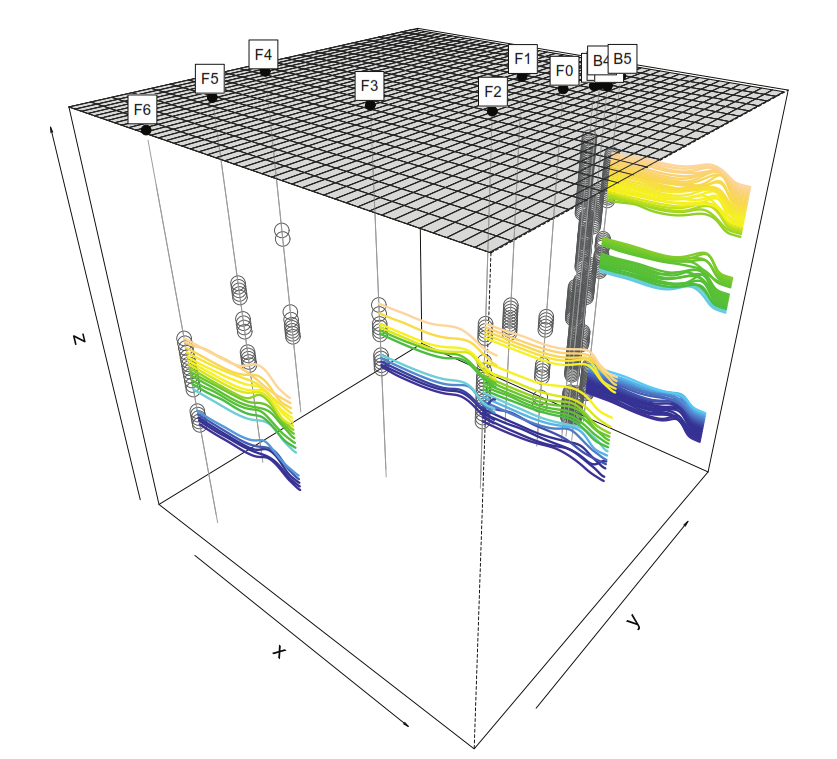
\includegraphics[width=8cm]{./pictures/psc/particle_size_densities.png}
	\centering
	\caption{Three-dimensional representation of particle-size densities at the Lauswiesen site. Grey points represent measurement locations, colored curves represent a subset of the dataset of PSCs. Colors indicate the depth of the sampling locations along the borehole.}
	\label{fig:boreholes}	
\end{figure}

The aquifer is made up by alluvial material overlain by stiff silty clay and underlain by hard silty clay. The site characterization has been based on stratigraphic information
collected at a set of monitoring and pumping wells.  \\
PSCs describe the local distributions of grain sizes within the aquifer system.
A set of twelve discrete sieve diameters (i.e., from a minimum of 0.063 up to 100.0 mm) were employed to reconstruct these curves by way of grain sieve analysis on soil samples, as in \ref{fig:sieve}.  

\begin{figure}
	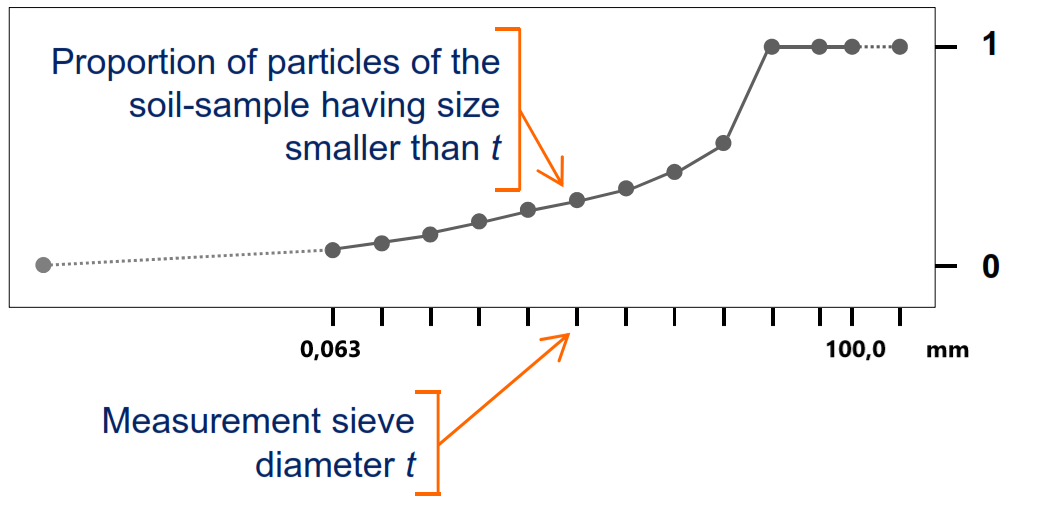
\includegraphics[height=3.5cm]{./pictures/psc/psc.png}
	\centering
	\caption{Example of particle-size raw data from sieze measurements, from clay and silt grains up to granules and pebbles.  \\
	We interpret PSCs as cumulative distribution functions and their derivatives as probability density functions. 
	Grain sieve analysis of soil samples, indeed, yields a discrete representation of the curves by measuring selected particle diameters which, in turn, correspond to quantiles of the particle-size curve.}
	\label{fig:sieve}	
\end{figure}

From the mathematical viewpoint, a particle-size density is a probability density function, associated with the distribution of particle sizes within a given soil sample. 

As such, available data consist of a set of constrained curves, spatially distributed. The statistical characterization of PSCs plays a key role in the classification of soil types, for inferring hydraulic parameters (e.g., porosity, permeability and hydraulic conductivity), and reconstructing the internal architecture of the groundwater system. 

In this vein, the study of PSCs may be concerned, as in \citep{menafoglio:psc}, with a geostatistical analysis, e.g. in order to identify clusters which represent the occurrence of different soil types and distinguish geomaterials at the site, and to characterize the spatial distribution of each identified textural class, and to provide Kriging estimates of the heterogeneous distribution of PSCs at unsampled locations. \\
Classification of aquifer geomaterials and estimation of their spatial arrangement is relevant to properly reconstruct the internal architecture of groundwater systems which can play a critical role in controlling contaminant spreading on different scales. 

As already pointed out, in the present case study an estimate of the particle-size curve at a given spatial location \textit{s} is available only for a set of \text{N} = 12 sieve diameters.  \\
To achieve any of the goals listed above, as in several other practical field situations, preprocessing of the raw data is required to obtain smooth estimates of the PSCs and associated densities.

The support of the PSCs has been assumed to be compact, upon setting the data support as \text{I} = $[\log(0.001),\log(200)]$, consistent with the type of lithology at the site.

Figure \ref{fig:psc_smoothed} depicts the resulting smoothed curves, obtained applying the algorithm described in chapter \ref{problem}.

\begin{figure}[ht]
	
	\begin{subfigure}{.5\textwidth}
		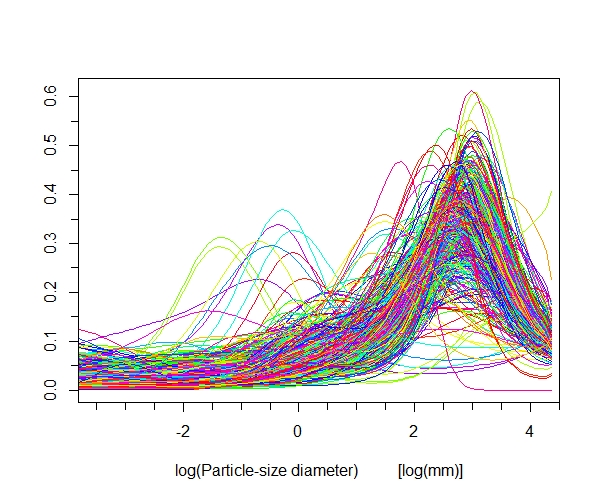
\includegraphics[width=6cm]{./pictures/psc/psc_all_res_4.jpeg} 
		\label{fig:subim1}
	\end{subfigure}
	\begin{subfigure}{.5\textwidth}
		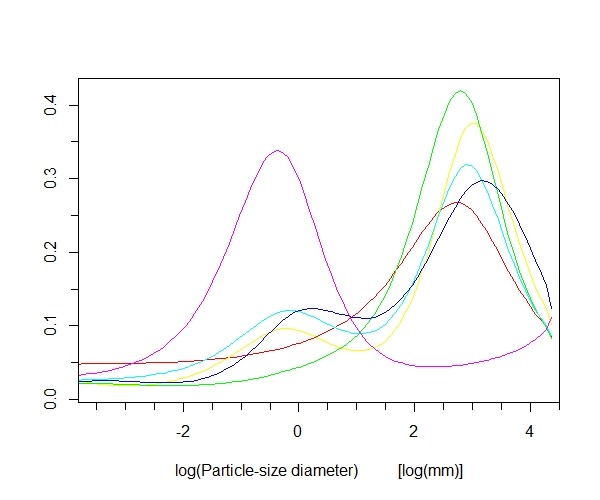
\includegraphics[width=6cm]{./pictures/psc/psc_few_res_4.jpeg}
		% \caption{Test C}
		\label{fig:subim2}
	\end{subfigure}
	
	\caption{Smoothed particle-size densities: on the left, all in one picture, and, on the rigth, just a few of them, chosen quite randomly, to highligth the variety in the soil composition for different sampling locations}
	\label{fig:psc_smoothed}
	
\end{figure}


%---------------------------------------------------------------
\section{Application to the well-known Iris flower data set}
The Iris flower data set is a multivariate data set introduced in the 1930s by Sir Ronald Fisher, who collected the data to quantify the morphologic variation of Iris flowers of three related species.
 
The dataset consists of 50 samples from each species of Iris flowers (Iris setosa, Iris virginica and Iris versicolor). Four features were measured from each sample, they are the length and the width of sepal and petal, in centimeters. 

We focus our attention on the variable related to the length of sepal, shown in figure \ref{fig:iris}.

\begin{figure}
	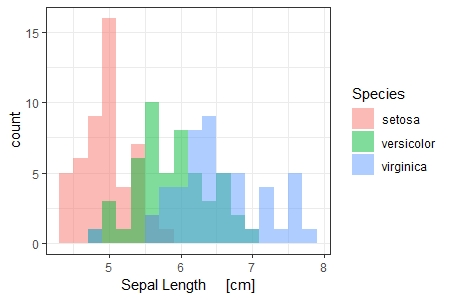
\includegraphics[height=3.5cm]{./pictures/iris/iris.jpeg}
	\centering
	\caption{Histogram of the variable Sepal Length for the Iris data set}
	\label{fig:iris}	
\end{figure}

The results are represented in figures \ref{fig:setosa} and \ref{fig:iris_v}: to be precise, the former shows how the algorithm works for different values of $\alpha$ when applied to the measures related to the Setosa species, the latter presents just the other two species for a fixed $\alpha$. 

It is worth remembering that the parameter is related to the fidelity term - the higher $\alpha$ is, the more the output density is forced to stay near to the given values of the histogram.

\begin{figure}[ht]
	
	\begin{subfigure}{.5\textwidth}
		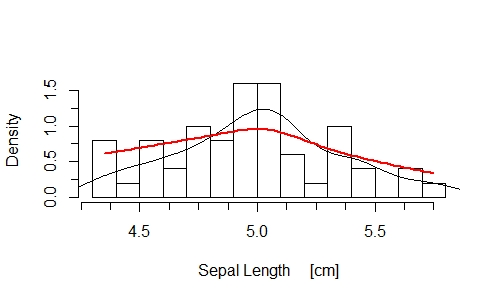
\includegraphics[width=6cm]{./pictures/iris/setosa_10.jpeg} 
		\caption*{$\alpha$ = 10}
		\label{fig:alpha10e1}
	\end{subfigure}
	\begin{subfigure}{.5\textwidth}
		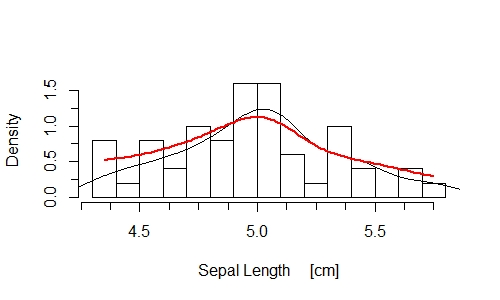
\includegraphics[width=6cm]{./pictures/iris/setosa_100.jpeg}
		\caption*{$\alpha$ = 100}
		\label{fig:alpha10e2}
	\end{subfigure}

	\begin{subfigure}{.5\textwidth}
		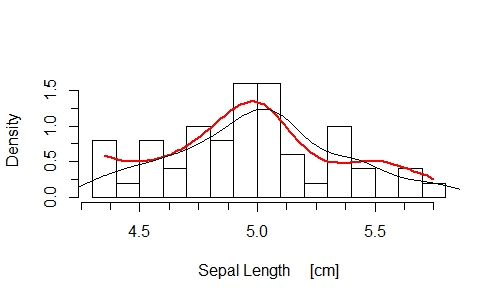
\includegraphics[width=6cm]{./pictures/iris/setosa_1000.jpeg} 
		\caption*{$\alpha$ = 1000}
		\label{fig:alpha10e3}
	\end{subfigure}
	\begin{subfigure}{.5\textwidth}
		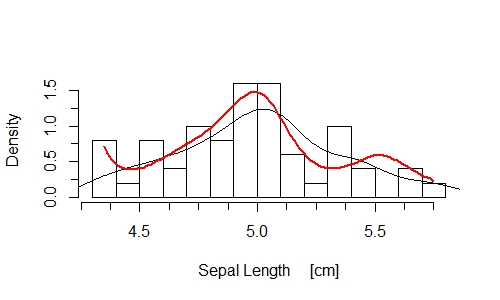
\includegraphics[width=6cm]{./pictures/iris/setosa_10000.jpeg}
		\caption*{$\alpha$ = 10000}
		\label{fig:alpha10e4}
	\end{subfigure}
	\caption{Data related to the Iris Setosa and the estimated density for different values of $\alpha$. The black line represents the "real" density, obtained from all the data through the kernel estimate. The coloured line is the density estimated with the algorithm - which is applied to the histograms.}
	\label{fig:setosa}
	
\end{figure}

\begin{figure}[ht]
	
	\begin{subfigure}{.5\textwidth}
		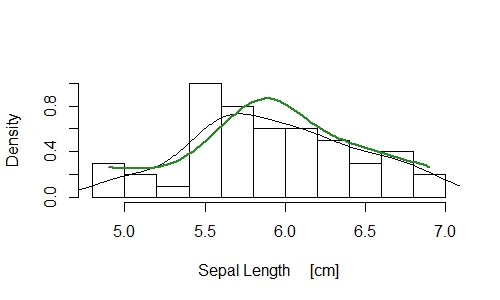
\includegraphics[width=6cm]{./pictures/iris/versicolor_100.jpeg} 
		\caption*{Iris Versicolor}
		\label{fig:versicolor}
	\end{subfigure}
	\begin{subfigure}{.5\textwidth}
		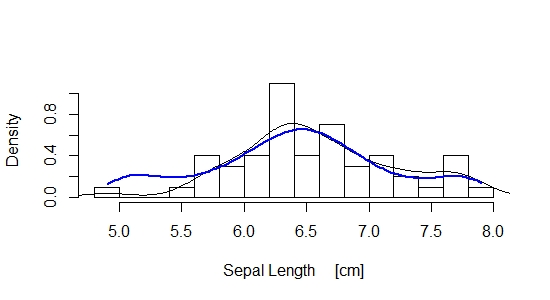
\includegraphics[width=6cm]{./pictures/iris/virginica_1000.jpeg}
		\caption*{Iris Virginica}
		\label{fig:virginica}
	\end{subfigure}
		
	\caption{Data related to the other two species of Iris. $\alpha$ is fixed and set to 1000.}
	\label{fig:iris_v}
	
\end{figure}




%---------------------------------------------------------------





\chapter{Installation}
\label{installation}
% \thispagestyle{empty}

\noindent 
The source code of this R package can be found and downloaded from \url{https://github.com/fpavone/pacs_spline_density} in the branch \textit{ROpenMP}. 
There are different ways of installing it on your machine.

The first one requires the use of \verb|devtools|, a popoular R package. It will also take care of installing all dependencies (Rcpp and RcppEigen) and install the splineDensity package in the same directories of all the other R packages installed.  \\
In R, use the command 
\begin{Verbatim}[commandchars=\\\{\}]
install_github("fpavone/pacs_spline_density",ref="ROpenMP")
\end{Verbatim}
Using \verb|devtools|, it's possible to install the package from the terminal.
Once the source code is downloaded and unzipped, it is enough to run from the package root folder the following commands:
\begin{Verbatim}[commandchars=\\\{\}]
   R -e \textcolor{red}{"library(devtools); install()"} --silent
\end{Verbatim}
To build the documentation in Roxygen, then:
\begin{Verbatim}[commandchars=\\\{\}]
   R -e \textcolor{red}{"library(devtools); document()"} --silent
\end{Verbatim}

This second command will create a subfolder named man where the .Rd files will be stored. This will be useful when calling for "help" from R (e.g., ?smoothSplines).

As an alternative, the second way to complete the installation does not require any additional package, but will throw errors if the packages required for the functioning of splineDensity are not installed.
From the terminal, you need to run:
\begin{verbatim}
   R CMD BUILD <path to folder splineDensity>
   R CMD INSTALL -l <path name of the R library tree> 
      <path name of the package to be installed>
\end{verbatim}

To test the successful installation of the package, it is possible to run one of the examples in the subdirectory tests, either from terminal
\begin{verbatim}
   Rscript <what-else-test.R>
\end{verbatim}
or directly in R.

To build the \verb|Doxygen| documentation of the C++ code instead, you need to navigate to the \textit{src} folder and type 
\begin{verbatim}
   doxygen -g <config-file>
\end{verbatim}
This will create a configuration file (if \verb|<config-file>| is missing, by default it will be named \textit{Doxyfile}), that can be edited to customize the output. \\
To run Doxygen then type:
\begin{verbatim}
   doxygen <config-file>
\end{verbatim}
To get the Reference Manual, then go to the \textit{latex} subfolder that has been generated and type \verb|make|.



%---------------------------------------------------------------

\section{How to enable OpenMP parallelization}
If your compiler supports OpenMP parallelization, once you have downloaded the splineDensity package, look for the \textit{Makevars} in the \textit{src} subfolder.\\
Set the \verb|OPENMP| macro defined in it to a non-empty value to activate the parallelization, e.g. \verb|OPENMP = 1|. By default, the option is disabled.

Now, follow the instructions as above to install the package. \\
Once finished, you have the opportunity to exploit the benefits that only a parallel implementation can provide.


% ---- Bibliography ----
\addcontentsline{toc}{chapter}{Bibliography}
\bibliographystyle{plain}
\bibliography{references}
%\nocite{*}

% \appendix

% \pagestyle{fancy} 
% \fancyfoot{}                                               
% \renewcommand{\chaptermark}[1]{\markboth{\appendixname\ \thechapter.\ #1}{}} 
% \renewcommand{\sectionmark}[1]{\markright{\thesection.\ #1}}         
% \fancyhead[LE,RO]{\bfseries\thepage}    
                                        
% \fancyhead[RE]{\bfseries\leftmark}    
% \fancyhead[LO]{\bfseries\rightmark}     
% \renewcommand{\headrulewidth}{0.3pt} 

% \chapter{Documentazione del progetto logico}
\label{appendiceA}
\thispagestyle{empty}

\noindent Documentazione del progetto logico dove si documenta il progetto logico del sistema e se \`e il caso si mostra la progettazione in grande del SW e dell'HW. Quest'appendice mostra l'architettura logica implementativa (nella Sezione 4 c'era la descrizione, qui ci vanno gli schemi a blocchi e i diagrammi).


\end{document}





